\chapter{Evaluation and Results}
\label{chapter:evaluation}

\section{Evaluation Design}
\label{sec:evaluation_design}

This chapter evaluates the performance and reliability of the proposed uncertainty-aware CEP framework under controlled missing data scenarios. The goal is to assess how well the system maintains event continuity when sensor streams are partially missing, reflecting real-world disruptions.

\subsection{Evaluation Overview}
The evaluation is structured around three key components:
\begin{enumerate}
    \item \textbf{Missingness Patterns:} Controlled data loss patterns are introduced to simulate uncertainty and partial observability.
    \item \textbf{Dataset and Scenario:} A real-world multi-sensor dataset is selected to represent a distributed cyber-physical environment.
    \item \textbf{Event Patterns and Predictors:} Defined CEP rules and prediction models are tested to analyse system-level behaviour.
\end{enumerate}



\subsection{Missingness Patterns}
\label{sec:missingness_patterns}

To evaluate reconstruction robustness under uncertainty, the experiments introduce controlled data loss through a hybrid missingness scenario applied at three loss levels (10\%, 20\%, 30\%). 
This scenario blends both random and structured missingness mechanisms to more realistically emulate disruptions observed in SoTS environments. 
Results are compared against two reference cases: an \textbf{Oracle} baseline (no missing data) and a \textbf{Structural Gap} baseline (irrecoverable data loss).

\begin{itemize}
    \item \textbf{Hybrid Missingness (Proposed):}  
    Combines two complementary mechanisms with equal probability:  
    (i) \textit{Random (MCAR)} removals, where individual readings are deleted independently to represent sporadic communication losses or packet drops; and  
    (ii) \textit{Block Missingness}, where consecutive readings (ranging from 2--6 hours) are removed to simulate short sensor outages or temporary twin disconnections.  

    \item \textbf{Structural Gap (Baseline):}  
    Represents long or permanent data absences due to known downtime, maintenance periods, or total node failure. These gaps are intentionally unreconstructed and serve as a lower-bound reference for assessing the of event detection under persistent loss.

    \item \textbf{Oracle (Baseline):}  
    Ideal condition with complete, uninterrupted data, used as the upper-bound benchmark for reconstruction accuracy and event-detection confidence.
\end{itemize}





\subsection{Dataset Description}
\label{sec:dataset_description}

The experiments use the Chicago Park District Beach Water and Weather Sensors dataset~\citep{chicago_beach_sensors_dataset}, which records hourly measurements for variables such as water temperature, turbidity, wave height, and wave period across multiple beaches along Lake Michigan. 
For this study, three representative sites are used: Calumet Beach, Montrose Beach, and 63rd Street Beach. 
Their geographical distribution along the shoreline (Figure~\ref{fig:results_beach_map}) makes them well-suited for modelling a SoTS scenario.

\begin{figure}[H]
\centering
\fbox{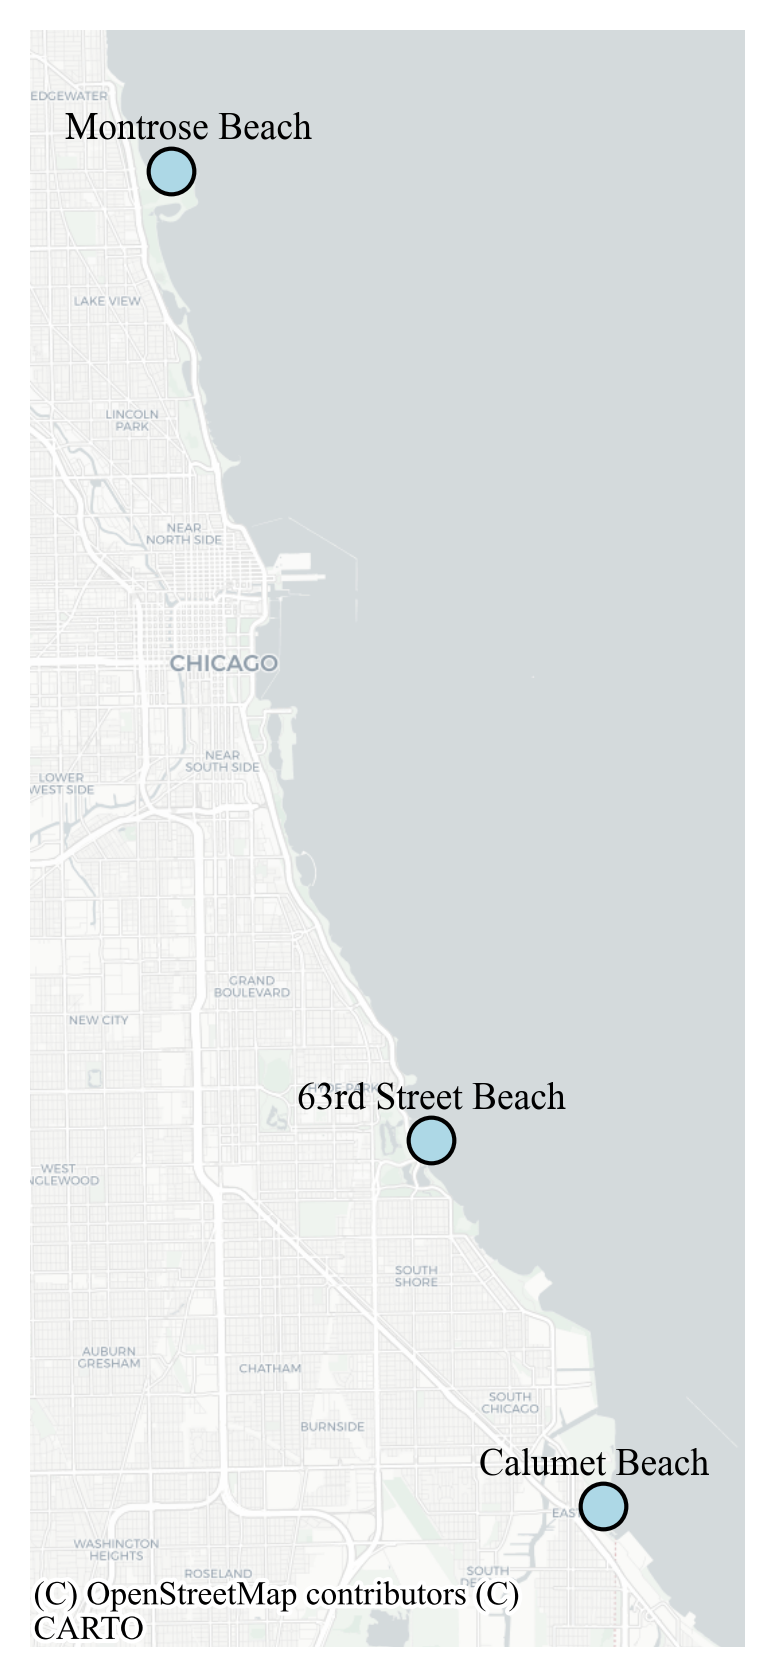
\includegraphics[width=0.45\textwidth]{figures/Results/beaches_map.png}}
\caption{Map of beaches}
\label{fig:results_beach_map}
\end{figure}


Each beach is modelled as a DT node continuously monitoring local water and environmental conditions. 
Together, these nodes form a distributed network that collectively represents the coastal monitoring system for safety monitoring and environmental awareness 

The beaches are located in adjacent regions, meaning that environmental changes, such as wave propagation, temperature shifts, or turbidity gradients, at one location can influence conditions at others. 
This interdependence captures the \textit{emergent behaviour} typical of SoS environments, where local phenomena have system-level impacts. 
In a realistic deployment, such a network could support autonomous actions, such as:
\begin{itemize}
    \item issuing public safety alerts for high bacterial or turbidity levels,
    \item coordinating automated water pumping or drainage responses during high wave events,
    \item dynamically adjusting sensor sampling rates based on neighbouring conditions.
\end{itemize}

Thus, the dataset provides a strong foundation for evaluating the framework in a realistic SoTS context.


\subsection{Dataset Statistics and Visual Overview}
\label{sec:results_dataset_visuals}

Figure~\ref{fig:results_attr_distributions_beach} presents the per-beach distributions of the key measured attributes, water temperature, turbidity, wave height, and wave period, during the 2015 summer season. 
These distributions capture the statistical variability observed at each site and highlight local environmental differences across the Chicago coastline. 
While the overall shapes remain consistent across beaches, subtle shifts in means and variances reflect their location differences influenced by shoreline shape, wave exposure, and localized weather conditions.

\begin{figure}[H]
\centering
\fbox{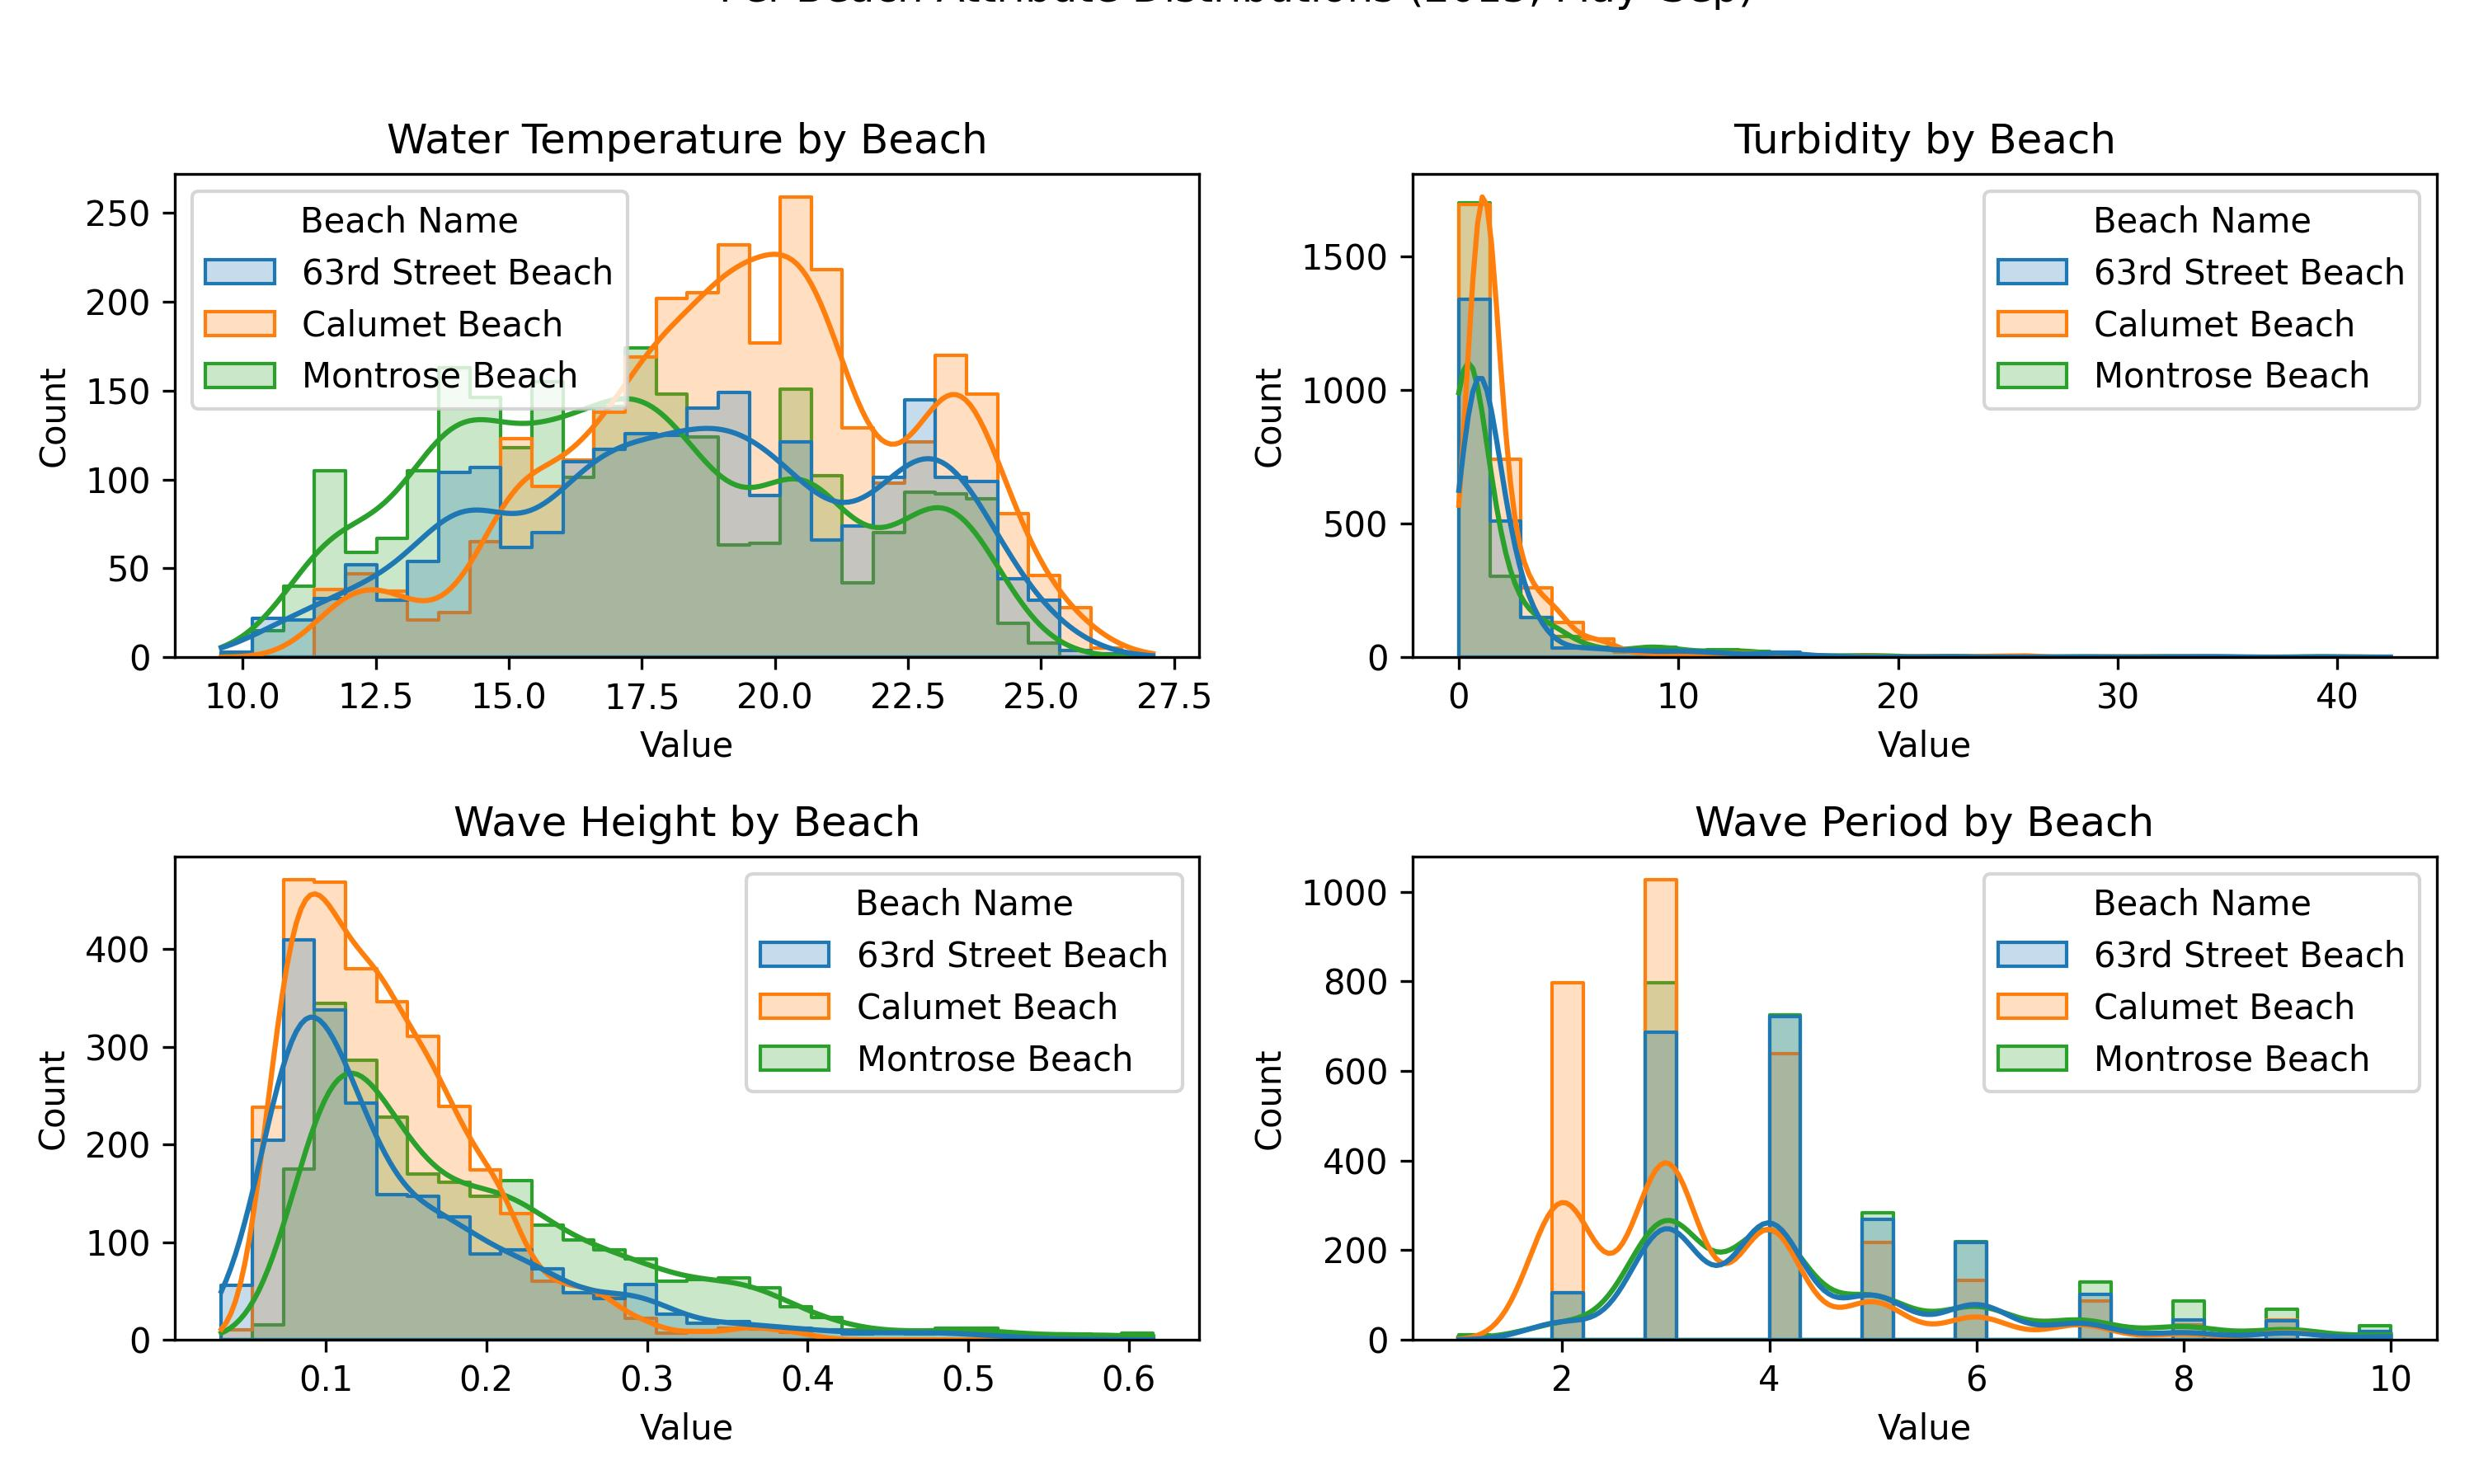
\includegraphics[width=0.85\textwidth]{figures/Results/attribute_histograms_per_beach_2015_5_9.jpg}}
\caption{Per-beach attribute distributions (May–September 2015).}
\label{fig:results_attr_distributions_beach}
\end{figure}

Figure~\ref{fig:results_time_series} provides a time-series overview for each beach. Water temperature exhibits gradual seasonal warming, while turbidity and wave-related attributes show irregular bursts corresponding to storm events, rainfall, or inflow disturbances. 

\begin{figure}[H]
\centering
\fbox{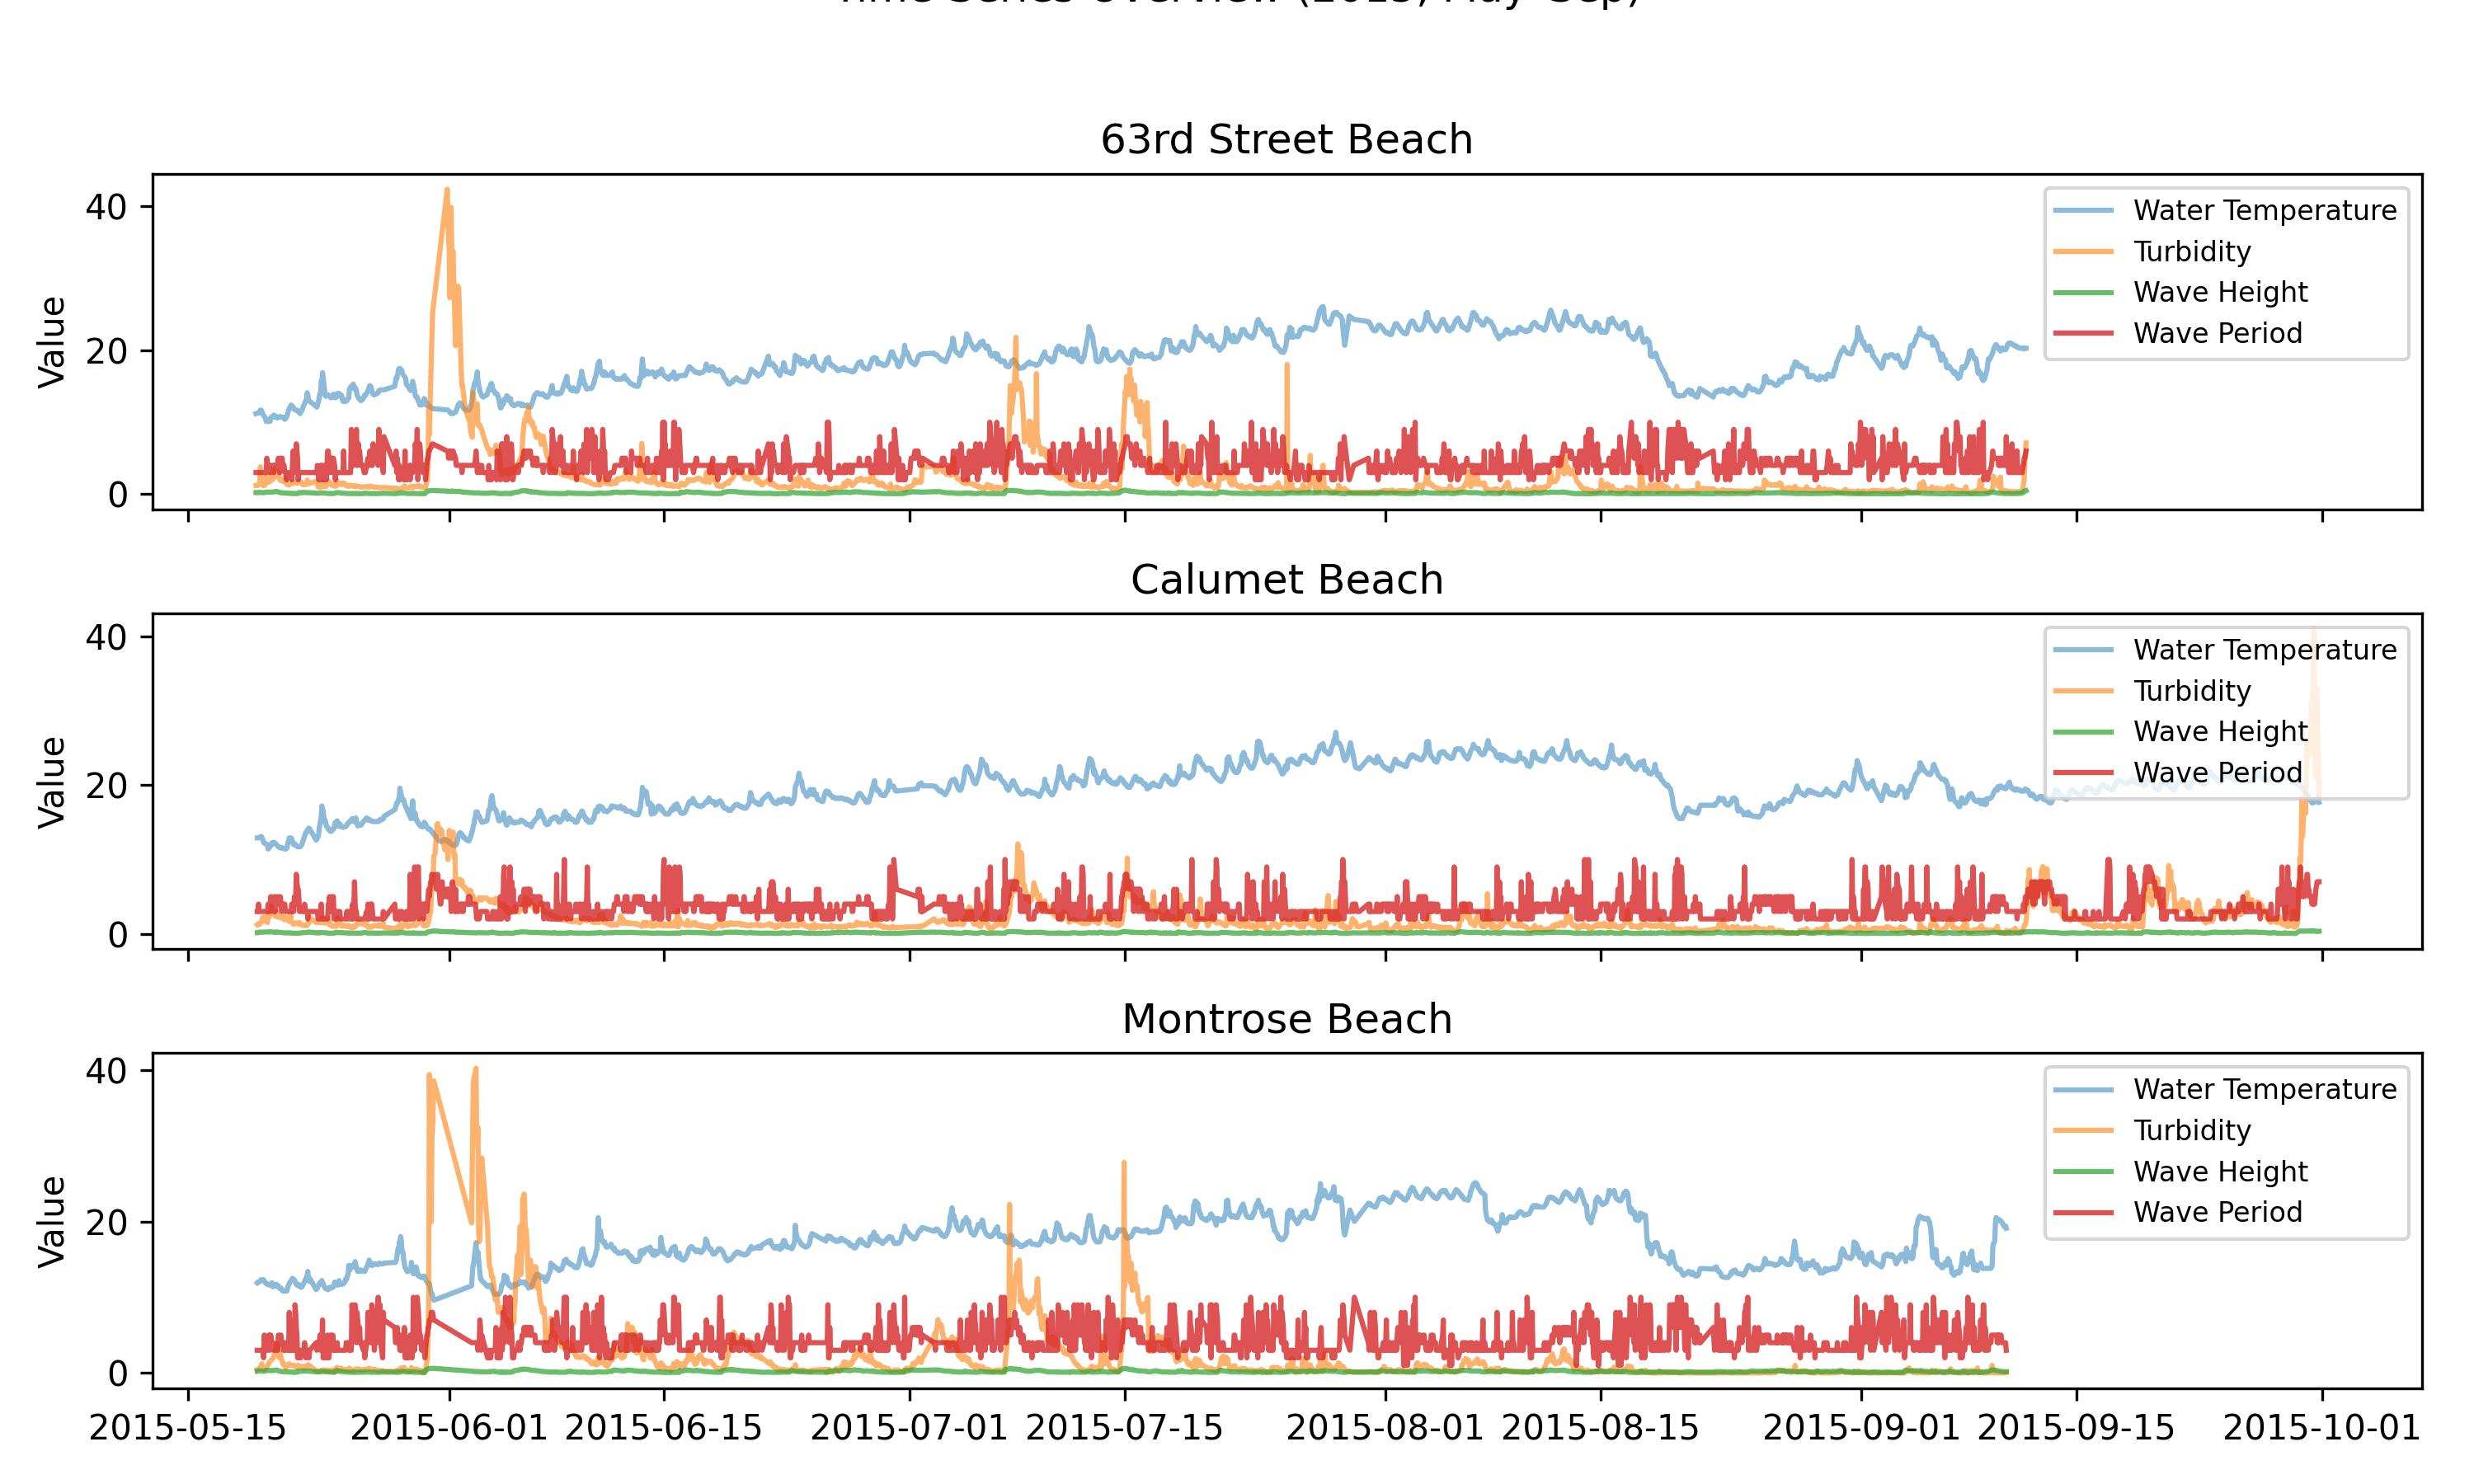
\includegraphics[width=0.9\textwidth]{figures/Results/time_series_overview_2015_5_9.jpg}}
\caption{Hourly time-series overview for the three selected beaches (May–September 2015).}
\label{fig:results_time_series}
\end{figure}









\subsection{Scenario Setup}
\label{sec:scenario_setup}

The experimental process follows the general workflow below:

\begin{itemize}
    \item Each beach node generates sensor readings at fixed hourly intervals, representing continuous monitoring of environmental parameters. 
    \item When data gaps occur, the system automatically estimates the missing values using the selected prediction model to maintain a consistent event flow. 
    \item Both the original and reconstructed data streams are then used for complex event detection, allowing the evaluation of how uncertainty and data loss influence overall system behaviour.
\end{itemize}




\subsection{CEP Evaluation and Event Patterns}
\label{sec:event_patterns}

To evaluate detection performance under uncertainty, the CEP layer was tested with varying confidence thresholds and hierarchical patterns. 

Each experiment was conducted using detection cutoffs of \textbf{0.65}, \textbf{0.75}, \textbf{0.85}, and \textbf{0.95}, enabling comparison across multiple confidence levels. These thresholds represent progressively stricter detection requirements, allowing analysis of system performance under relaxed, moderate, and highly selective confidence conditions.


The evaluation uses hierarchical set of patterns, progressing from simple sensor-level conditions (atomic events) to beach-level (local complex) and system-wide (distributed complex) alerts. 
This structure reflects the SoTS concept: local twins operate autonomously but can trigger collective behaviour when multiple conditions align across nodes. 
For all complex patterns, event confidence is computed as the \textbf{mean confidence} of the constituent events that make them up.

\begin{figure}[H]
\centering
\fbox{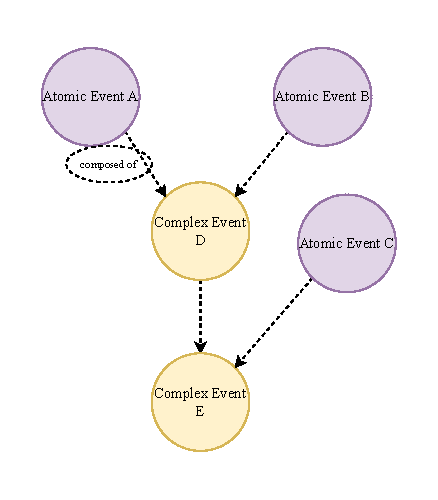
\includegraphics[width=0.45\textwidth]{figures/Results/Results Patterns.drawio.pdf}}
\caption{Illustration of a sample event composition of atomic and complex events}
\label{fig:event_composition}
\label{fig:results_pattern_composition}
\end{figure}



\begin{table}[H]
\centering
\caption{Hierarchy of event patterns used in the evaluation.}
\label{tab:event_patterns}
\renewcommand{\arraystretch}{1.1}
\begin{tabular}{p{0.18\textwidth} p{0.22\textwidth} p{0.53\textwidth}}
\toprule
\textbf{Event Type} & \textbf{Example Name(s)} & \textbf{Condensed Description} \\
\midrule

\textbf{Atomic (Sensor-level)} 
& \texttt{HighTurbidity}, \texttt{LowWaterTemp}, \texttt{HighWave}, \texttt{HighWavePeriod}
& Single-sensor threshold events per beach, such as turbidity $>$ 8.5\,NTU, wave height $>$ 0.35\,m, or temperature $<$ 22°C. These serve as the building blocks for higher-level detection. \\

\textbf{Local Complex (Beach-level)} 
& \texttt{LocalAlert}
& Combines two atomic events within the same beach (e.g., high turbidity and low temperature at Calumet, or high turbidity and high wave height at Montrose) occurring within 3\,s. Represents short-term local correlations indicative of abnormal conditions. \\

\textbf{Distributed Complex (Cross-beach)} 
& \texttt{AlertSpread}, \texttt{TripleAlert}
& Captures inter-beach propagation of alerts (e.g., Montrose $\rightarrow$ Calumet $\rightarrow$ 63rd) within short windows (5–7\,s). Reflects emergent regional SoTS behaviour, where local anomalies align across multiple sites. \\

\bottomrule
\end{tabular}
\end{table}


\subsection{Predictor Configuration}
\label{sec:predictor_configuration}

Two predictors were chosen to evaluate the reconstruction of the missing sensor readings: the Kalman Filter (KF) and the Particle Filter (PF).  

\noindent\textbf{Kalman Filter.}  
The Kalman Filter is a recursive state estimator that models the evolution of a variable as a linear dynamical system with Gaussian noise.  
At each step, the filter predicts the next state based on the previous estimate and corrects it when a new measurement becomes available, balancing process and measurement uncertainty through their respective covariances.  

Confidence is computed using the covariance trace, which quantifies how the current uncertainty compares to the filter's initial uncertainty. 
It is derived directly from the posterior covariance matrix of the Kalman filter and defined as:

\begin{equation}
    \text{confidence}_{\text{KF}} 
    = 1 - \frac{\operatorname{trace}(P_k)}{\operatorname{trace}(P_0)}
\end{equation}

where $P_k$ denotes the posterior covariance matrix at the current time step, and $P_0$ represents the initial covariance matrix used for normalization. 
A lower trace value indicates reduced overall uncertainty, leading to higher confidence, whereas an increasing trace reflects the accumulation of uncertainty over time.

\paragraph{Rational} The confidence formula used is derived directly from the Kalman filter’s posterior covariance, which represents the estimator’s internal measure of uncertainty. Minimizing this quantity is equivalent to minimizing the mean-squared estimation error, making it a good basis for quantifying estimator precision. Building on the analysis of \citet{kang2021some}, who characterize the magnitude and decay of the Kalman filter’s error covariance as quantitative descriptors of uncertainty, the normalized covariance trace captures the overall reduction of uncertainty as the filter converges.



\vspace{0.5em}
\noindent\textbf{Particle Filter -}  
The Particle Filter approximates the posterior distribution through a set of weighted samples (particles) that evolve under the process model.  
Each particle represents a potential system state, with weights updated when new measurements arrive.  
When data are missing, particles propagate without correction.  
The Particle Filter used in this work follows the Sampling Importance Resampling (SIR) described by ~\citet{arulampalam2002tutorial}.

Confidence is computed from the spread of particles:
\[
\text{confidence}_{PF} = \frac{1}{1 + \text{Var}(\boldsymbol{p})}
\]
where \(\boldsymbol{p} = \{p_1, p_2, \ldots, p_N\}\) denotes the set of particles representing possible realizations of the system state. The variance of this distribution reflects the uncertainty in the estimated state: a tightly clustered particle set indicates high confidence, while a wide spread corresponds to greater uncertainty.

\paragraph{Rational} The confidence formula used ...


\subsubsection{Configuration and Initialization} 
\label{sec:predictor_config}

All predictors were tuned through a grid search using data from a subset of the dataset, Montrose Beach dataset (2016), which was excluded from subsequent evaluation. 
The tuning process simulated a baseline of 30\% missingness under an MCAR pattern to represent moderate uncertainty conditions. 
Parameter selection was guided by minimizing the Root Mean Squared Error (RMSE) between reconstructed and observed values, while simultaneously promoting a negative correlation between reconstruction error and model confidence. In other words, low-accuracy predictions were expected to return lower confidence, and high-accuracy predictions higher confidence.

A combined score function was used to balance these two criteria:

\begin{equation}
\label{eq:gridsearch_score}
S = \alpha \cdot \mathrm{RMSE} + (1 - \alpha) \cdot (1 - \rho),
\end{equation}

where \( \rho \) denotes the Pearson correlation between the model’s confidence estimates \(c_t\) and the corresponding reconstruction errors \(|y_t - \hat{y}_t|\). 
The weighting factor \(\alpha = 0.75\) prioritizes reconstruction accuracy while still rewarding consistent confidence outputs. 






\begin{table}[H]
\centering
\caption{Grid search parameter ranges for predictor tuning (Montrose Beach, 2016).}
\label{tab:predictor_params}
\begin{tabular}{lcc}
\toprule
\textbf{Predictor} & \textbf{Parameter} & \textbf{Range Tested} \\
\midrule
Kalman Filter & Process noise \(Q\) & [0.001, 0.005, 0.01, 0.05, 0.1, 0.2, 0.5, 1.0, 2.0] \\
              & Measurement noise \(R\) & [0.001, 0.002, 0.005, 0.01, 0.02, 0.05, 0.1, 0.2] \\
\midrule
Particle Filter & Process std. \(\sigma_Q\) & [0.001, 0.005, 0.01, 0.05, 0.1, 0.2, 0.3] \\
                & Measurement std. \(\sigma_R\) & [0.002, 0.005, 0.01, 0.02, 0.03] \\
                & Number of particles \(N_p\) & [100, 250, 500, 750, 1000] \\
\bottomrule
\end{tabular}
\end{table}



All predictors were initialized using the minimum observed value of each variable from the 2016 dataset and fixed with the optimal configurations identified through the grid search.  





% -------------------------------------------------------------
\section{Results}
\label{sec:results}

This section presents the quantitative and qualitative results of the evaluation, comparing reconstruction quality and complex event detection accuracy across the oracle, MCAR, and structural-gap conditions.

\subsection{Reconstruction Accuracy}

\begin{table}[H]
\centering
\caption{Comparison of reconstruction performance (MAE) per dataset and attribute (averaged across beaches) between Kalman and Particle filters under hybrid missingness.}
\label{tab:recon_mae_per_dataset_attribute_comparison}
\resizebox{\textwidth}{!}{%
\begin{tabular}{lccccccc}
\toprule
\multirow{2}{*}{Attribute} & \multicolumn{3}{c}{\textbf{Kalman Filter}} & & \multicolumn{3}{c}{\textbf{Particle Filter}} \\
\cmidrule(lr){2-4} \cmidrule(lr){6-8}
 & hybrid\_10 & hybrid\_20 & hybrid\_30 & & hybrid\_10 & hybrid\_20 & hybrid\_30 \\
\midrule
Turbidity         & \textbf{0.037} & \textbf{0.090} & \textbf{0.141} & & X & X & X \\
Water Temperature & \textbf{0.032} & \textbf{0.073} & \textbf{0.122} & & X & X & X \\
Wave Height       & \textbf{0.002} & \textbf{0.005} & \textbf{0.007} & & X & X & X \\
Wave Period       & \textbf{0.117} & \textbf{0.241} & \textbf{0.337} & & X & X & X \\
\bottomrule
\end{tabular}%
}
\end{table}


\subsection{Event Continuity and Detection}
\subsubsection{Kalman Filter}


\subsection{Confidence Behavior}
(Plots of confidence trajectories under varying $Q$ and missingness rates.)

\subsection{System-Level Observations}
(Summarize emergent patterns across all beaches — e.g., correlation, stability, and temporal drift.)


